\chapter{Background}
\label{ch:background}

% http://www.ccs.neu.edu/home/will/CPP/dangling.html has a good example of a dangling pointer error leading to double delete

\section{Virtual memory}

Virtual memory is an abstraction over the physical memory available to the hardware. It's an abstraction that is typically transparent to both the applications and developers, meaning that they do not have to be aware of it, while enjoying the significant benefits. This is enabled by the hardware and operating system kernel working together in the background.

From a security and stability point of view, the biggest benefit that virtual memory provides is address space isolation: each process executes as if it was the only one running, with all of the memory visible to it belonging either to itself or the kernel. This means that a malicious or misbehaving application cannot directly access the memory of any other process, to either deliberately or due to a programming error expose secrets of the other application (such as passwords or private keys) or destabilize it by corrupting its memory.

An additional security feature is the ability to specify permission flags on individual memory pages: they can be independently made readable, writeable, and executable. For instance, all memory containing application data can be marked as readable and writeable, but not executable, while the memory pages hosting the application code can be made readable and executable, but not writeable, severely limiting the capabilities of attackers.

Furthermore, virtual memory allows the kernel to optimize physical memory usage by:

\begin{itemize}
	\item Compressing or swapping out (writing to hard disk) rarely used memory pages (regions) to reduce memory usage
	\item Deduplicating identical memory pages, such as those resulting from commonly used static or shared libraries
	\item Lazily allocating memory pages requested by the application
\end{itemize}

Virtual memory works by creating an artificial (virtual) address space for each process, and then mapping the appropriate regions of it to the backing physical memory. A pointer will reference a location in virtual memory, and upon access, is resolved (typically by the hardware) into a physical memory address. The granularity of the mapping is referred to as a memory page, and is typically 4096 bytes (4 kilobytes) in size. (See Figure~\ref{fig:virtual_memory})

\begin{figure}
	\centering
	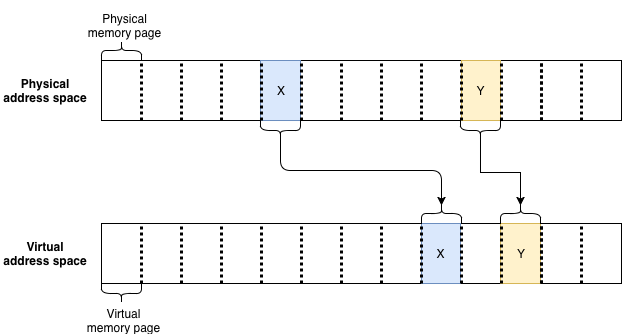
\includegraphics[width=\textwidth]{diagrams/virtual_memory.png}
	\caption{Mapping two physical memory pages X and Y to virtual memory}
	\label{fig:virtual_memory}
\end{figure}

This mapping is encoded in a data structure called the \emph{page table}. This is built up and managed by the kernel: as the application allocates and frees memory, virtual memory mappings have be created and destroyed. The representation of the page table varies depending on the architecture, but on x86-64, it can be represented as a tree, with each node an array of 512 page table entries of 8 bytes each making up a 4096 byte page table page. The root of this tree is where all virtual memory address resolution begins, and it identifies the address space. The leaf nodes are the physical memory pages that contain the application's own data.
The bits of the virtual memory address identify the page table entry to follow during address resolution. For each level of page tables, 9 bits are required to encode an index into the array of 512 entries. Each entry contains the physical memory address of the next page to traverse during the address resolution. Finally, the least-significant 12 bits are used to address into the application's physical page (which is 4096 bytes) itself and so require no translation. (See Figure~\ref{fig:page_table_tree})

On x86-64, there are currently 4 levels of page tables, using $4 * 9 + 12 = 48$ out of the 64 available bits in the memory addresses, and limiting the size of the address space to $2^{48}$ bytes or 256 terabytes. (The size of addressable space per page table level, in reverse resolution order being: $512 * 4$ kilobytes = 2 megabytes; $512 * 2$ megabytes = 1 gigabyte; 512 gigabytes; 256 terabytes.)

\begin{figure}
	\centering
	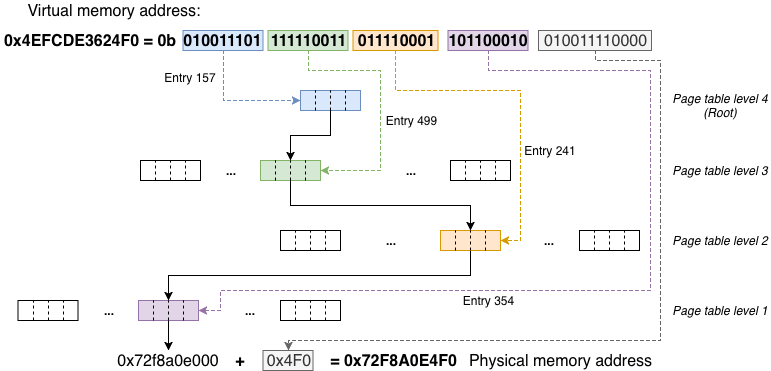
\includegraphics[width=\textwidth]{diagrams/page_table_tree.png}
	\caption{Translating a virtual memory address to physical using the page tables}
	\label{fig:page_table_tree}
\end{figure}

Note that it is possible to map a physical page into multiple virtual pages, and it is also possible to have unmapped virtual pages. Attempting to access a virtual page that is not mapped (i.e. not backed by a physical memory page) will cause execution to trap inside the kernel, which will then usually interpret it as segmentation fault and kill the process. (This is also how lazy memory allocation and swapping out works: instead of killing the process, the kernel goes ahead and allocates the physical memory it promised, or swaps the page back in from disk.)

Thanks to Dune, Dangless has direct access to the page tables, and manipulates them using custom functions (see \textit{include/dangless/virtmem.h} and \textit{src/virtmem.c}). Upon memory allocation, Dangless forwards the allocation call to the system allocator and then reserves a new virtual page, mapping it to the same physical address as the a virtual page returned by the system allocator. This is called virtual aliasing. During deallocation, besides forwarding the call to the system allocator, Dangless unmaps the virtual alias page and overwrites the page table entry with a custom value, enabling it to recognize a would-be access through a dangling pointer.

\section{Prior art}

\todo{Oscar, etc.}
